
\section{System Overview of \toolNew} \label{subsec:motivate_eg}

%Then, we explain the basic idea of our proposed solution and sketch the system overview.
%srj
%aum gaanathipathaye namaha
%\section{BinGo System Overview}\label{sec:overview}
%\note{not done - will do last after reviewing all other sections}
%compiler, architecture and OS agnostic
%\vspace{-3mm}
\begin{figure}[t]
\begin{center}
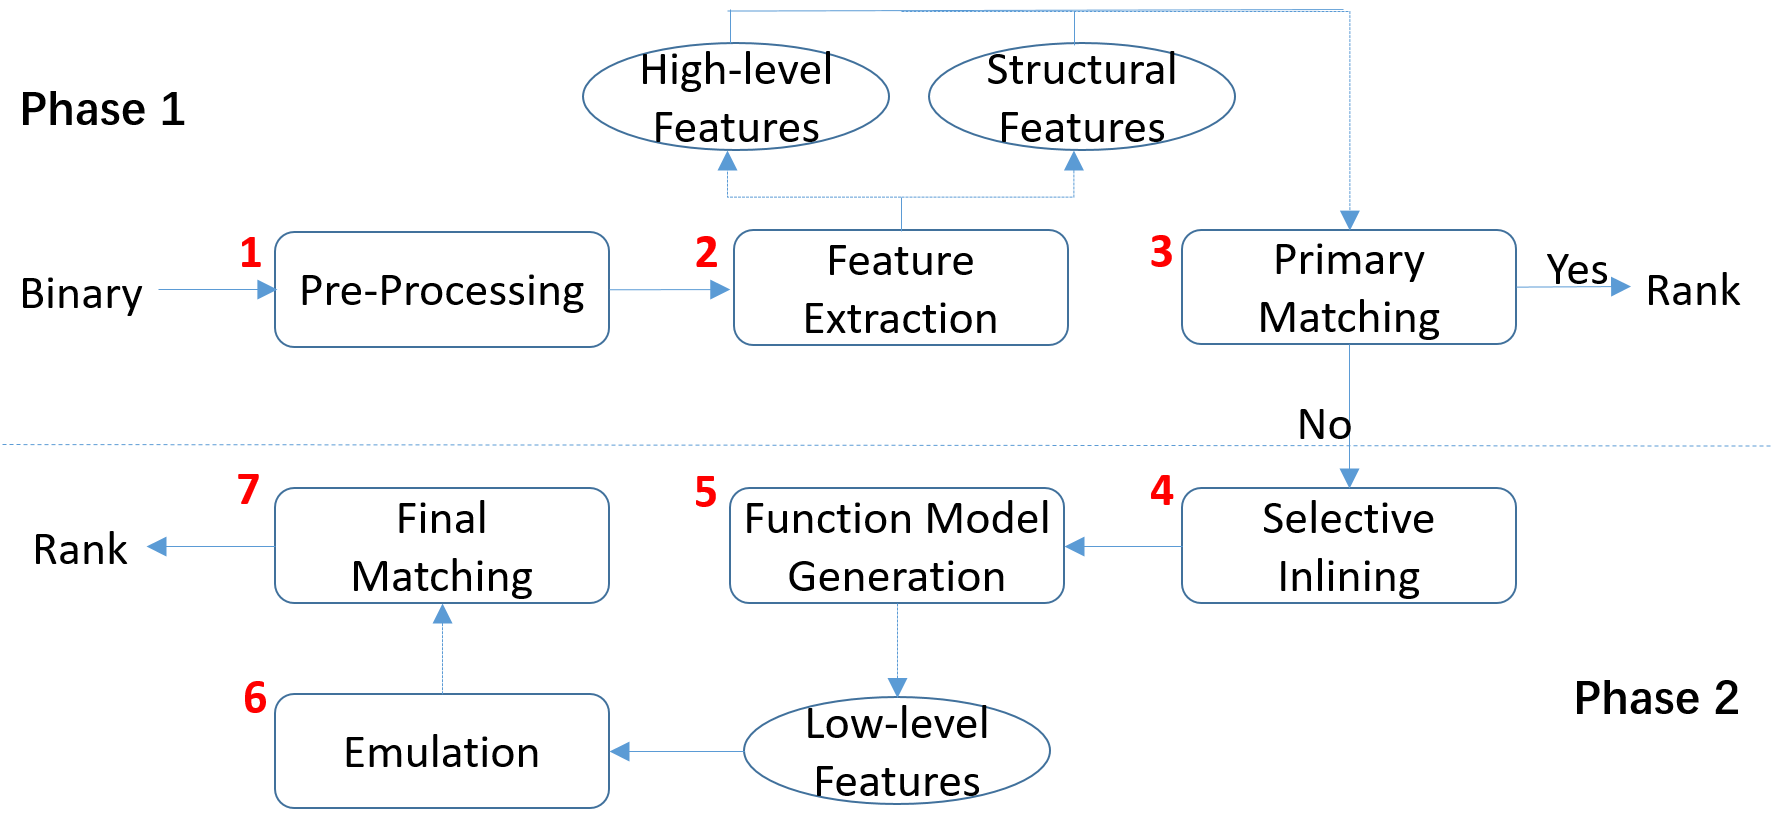
\includegraphics[width=9cm]{srj-figures/bingo_e_arch.png}
\caption{\toolNew work flow: rectangles represent processing steps, ovals represent features, arrows represent control/data flows}
\label{fig:archi}
\end{center}
\end{figure}

\toolNew, as a new extension of \tool, aims to be an accurate and scalable search engine for binary code. Given a binary function to be matched (\emph{signature function} in search), \toolNew returns the functions from the pool of analyzed binaries (\emph{target function} in search), ranked based on their semantic similarity.

\subsection{The Sketch of Work Flow} \label{subsec:workflow}
% Table generated by Excel2LaTeX from sheet 'Sheet1'

Fig.~\ref{fig:archi} shows the work flow of \toolNew. The input is one signature binary function and the possible candidate target functions. The output is the ranked list of candidate target functions above the user-defined threshold of similarity score. %, namely, pre-processing, selective inlining, filtering, partial trace generation, function model generation and similarity matching.
The basic idea is the two-phase matching: first employing the structural and high-level semantic features to find similar target functions;
if the similarity scores of all the returned target functions are below a certain threshold (\emph{No} flow after primary matching in Fig.~\ref{fig:archi}),  adopting the low-level semantic features to compare the I/O values on  $k$-tracelets of the signature function with those of candidate target functions.

We explain how each step in our approach works in brief. At step 1, given a signature function, it performs the preprocessing, i.e., disassembling  and building the CFG for the signature function.
At step 2, we extract these features from the high-level semantics and structure information in Table~\ref{tab:features}. \xyx{As shown in Table~\ref{tab:features}, we extract 6 types of high-level semantic features (\S\ref{sec:category:highSemanticFea}) and 3D-CFG structural features (\S\ref{sec:category:structralFea}).}
At step 3, \xyx{a primary matching step is conducted to measure the similarity  based on the Jaccard distance of high-level semantic features and the centroid distance of structural features (\S\ref{subsec:matching:primary})}.
If no results are above the similarity threshold, the process proceeds with comparing low-level semantic features (\S\ref{subsec:matching:lowFea}). At step 4, for each function in the target binaries, function calls are identified and selectively inlined according to the relevance of called libraries and other user-defined functions (\S\ref{sec:inline}). \xyx{Note that selective inlining is for addressing C2 (\S\ref{subsec:sem_chall}). Selective inlining is transitive. Assume function $a$ calls function $b$ and $b$ calls function $c$. If $a$ selectively inlines  $b$, then the decision of inlining $c$ into  $b$ is according to Algorithm \ref{algo:select-inline} (\S\ref{sec:inline}). If $a$ does not need to inline $b$, then it is certainly unnecessary to inline $c$ into  $b$.}
%Then from these inlined target functions, we shortlist a list of candidate functions that are similar to the signature function by using three filters, which consider different aspects of the binary semantic (\S\ref{sec:prefilter}). %, where at the end of filtering process, \tool returns a list of target functions that are similar to the signature function.
%It is noted that selective inlining (Section~\ref{sec:inline}) is carried out as part of filtering process.
At step 5, for the signature functions, length variant partial traces (up to $k$-tracelets) are generated  and grouped to form the function models (\S\ref{subsec:partial_trace_ext}), which  low-level semantic features are extracted from (\S\ref{subsec:fun_mod_mat}). %(\S\ref{subsec:sem_fea_ext}), and these features are later used for semantic similarity matching.
%Note that for candidate target functions, the process to function model generation, which just needs to be carried out for once, has been completed before.
Note that function model generation and feature extraction is a one-time job.
At step 6, we rely on emulation to get the input/output values, flags, memory addresses of signature functions as low-level semantic features (\S\ref{sec:emulation}).
Finally, at step 7, combining \xyx{Jaccard Distance} for low-level semantic features and results of the primary matching, \toolNew returns target functions that are above the similarity threshold in a ranked order (\S\ref{subsec:matching:final}). %, where rank \#1 is the \xyx{best} match to the signature function.

%The structure of following sections is:
The approach is presented in the following way: in \S\ref{sec:category}, different categories of features and emulation (step 2 and 6) are introduced; in \S\ref{sec:inline}, selective inlining (step 4) is elaborated; in \S\ref{sec:func_match}, the key steps 3, 5 and 7 are explained with details. %\S\ref{sec:experiemntation} presents evaluation results; \S\ref{sec:related} reviews the literatures; and \S\ref{sec:concl} concludes the paper.

%\tool will generate funIt is noted that to selective inlining is performed on all the target fucntions to extract


%\mahin{I didn't explain each of the modules here, either we can bring section 2.4 (proposed solution) here, or move this to sec 2.4 }

% and post-processing module.
%Given a binary program, \tool will first dissemble it into REIL intermediate representation (REIL IR).
%
%In the feature extraction module, two types of semantic features are extracted from partial execution traces: semantic features and structural features. State-base semantic features (see Section~\ref{subsec:stat_sem}) represent the low-level effects of executing the binary code in terms of machine state (i.e., characterised by register, condition-code flag and memory values) at various program points.
%Semantic features of API idioms (see Section~\ref{sec:idiom:def}) capture the OS dependent semantics of the binary code.
%Secondly, structural features and compiler idioms (see Section~\ref{sec:idiom:def}) can help to quickly find the binary code with similar program structural or representations.
%These features complementarily summarize the behaviour of binary code at various granularity levels, providing a comprehensive view to overcome the differences at syntax and structural levels. This is the one of the key contributions of this work for achieving accurate yet robust matching results.
%%In generating partial execution traces, we employ a \textit{pruning} technique that removes infeasible executions soundly, with the help of a theorem prover.
%
%In the function model generation module, for each function, a number of \textit{function models} are generated based on different combinations of partial traces.  Specifically, partial execution traces of various lengths are combined in different ways to represent the function models that account for structural changes in the compiled code, such as function inlining and outlining introduced by the compilers. For a given function, if partial traces of $n$ different lengths are generated, the function can be represented by $2^n-1$ different function models.
%
%Finally, the machine learning module applies feature hashing techniques on functions models, generated from each function, where they are put into `bins' based on their proximity to each other. That is, function models that are similar, in terms of syntax and semantic features, will likely to get into the same bin. Hence, for a given search query, using feature hashing, the appropriate bin is located and the matching functions are obtained from there. This improves searching time.

%Finally, post-processing module removes the outliers and variants of the same function in the search results, to improve the overall search ranking. For example, given two variants of the same function (e.g., \texttt{strncpy\_ia32} and \texttt{strncpy\_sse}) in the search results (e.g., assume \texttt{strncpy\_ia32} is ranked 1 and \texttt{strncpy\_sse} is ranked 2), only the highest ranking function (\texttt{strncpy\_ia32}) is kept in the search results and others are removed from it.


%In the following sections, we shall discuss the four modules in details.
%In practise, security analysts get to know about new vulnerabilities from a patch or a CVE advisory and, using the features (or characteristics) extracted from the known vulnerability (called, \textit{signatures}), try to find similar vulnerabilities in the programs they are interested in or concern about (called, \textit{target programs}).

%As can be seen in figure \ref{fig:overview}, our system consists of two phases, a pre-processing phase and a vulnerability signature matching phase. In preprocessing phase, we pre-process the program binaries for our vulnerability signature matching. In this phases, we first, disassemble the binary program and extract the control-flow structures. Then, synthetic features (i.e., code properties) are extracted from the disassembled functions. Next, each function is modelled using \textit{tracelet models}, where tracelet (explained in section \ref{subsec:vul_mod}) is a sequence of $n$ adjacent basic-blocks. Finally, from each tracelet model, the semantic features are extracted. It is important to note that the pre-processing only has to happen once per signature and target program. The pre-processed output can be reused in the future, for new vulnerability searches.


%In the vulnerability signature matching phase, our system searches for a signature within a target program and identifies binary code parts which are similar to the vulnerability signature. First, we first quickly search the target binary, using the synthetic features (i.e., code properties), to identify candidate functions (i.e., potentially vulnerable) in the target program . This pre-filtering process is cheap in terms of computational cost and considerably improves the scalability, where it reduces the number of `potentially' vulnerable functions from several thousands to few hundreds (sometimes even smaller), in the target program. Next, we compare the signature program against the selected candidate target functions using semantic features extracted in the pre-processing phase. To this end, we use the \textit{symbolic expressions} (explained in section \ref{subsec:sem_fea}, at high-level, it represents the effect of a piece of code on the program-state), extracted from the signature tracelet models and compare them with the symbolic expressions, extracted from the target tracelet models.
%Here, it is worth mentioning that $k_s$ take a single value, i.e., we fix the length of the tracelet for vulnerability signature (e.g., $k_s=3$), whereas $k_t$ takes a range of values starting from $1$ upto $n$ ($k_t\in\mathbb Z_{> 0}$), i.e., for a given bug signature, we try to match tracelets of various lengths, in the target function,  and choose the tracelet that is close to the signature in-terms of semantic similarity.

%Here, it is worth mentioning that the length of tracelets, for both signature ($k^s$) and target ($k^t$) programs, takes a range of values starting from $1$ upto $n$, where $n\in\mathbb Z_{> 0}$. For example, given a signature tracelet of size 2 (i.e., $k^s=2$), we try to match tracelets of various lengths (e.g., $k_s=1,2,3$), in the target function, and choose the tracelet that is closest to the signature in-terms of semantic similarity (i.e., \textit{optimal} tracelet model). In this way, we introduce self-adaptability in modelling the vulnerability, which allows us overcome the challenges, such as vulnerability models being sensitive to basic-block \textit{splitting} and \textit{merging}, prevailed in the vulnerability modelling techniques reported in the literature \cite{pewnycross}\cite{ruttenberg2014identifying}. Finally, at the end of the workflow, our system reports the similarity matrix, revealing the optimal tracelet models (i.e., optimal values for $k^s$ and $k^t$) for signature and target programs that maximize the tracelet similarity. From this, we can identify the target functions that are similar to the vulnerability signature and the optimal tracelet models, for both signature and target programs, that better represent the vulnerability.
 %~\xyx{In step 5, to facilitate cross-architecture analysis, to address the syntax differences of instructions, we lift the low-level assembly instructions into a corresponding intermediate representation (IR) and extract low-level semantic features based on that.}
%To mitigate C1 (the single basic block matching to several basic block matching in Fig.~\ref{fig:prob_stat})), we borrow the idea of tracelet used in \textsc{\small Tracy}~\cite{DBLP:conf/pldi/DavidY14}. Different from the original approach that uses a fixed length of tracelet, we use length variant partial traces. %to mitigate the effect of program structure distortion especially basic block structure.
%Next, to overcome C2 (e.g., whether to inline \texttt{memcpy} in Fig.~\ref{fig:prob_stat}(a)), we propose a selective inlining strategy to strike a balance between the needed contextual semantics and the overheads due to inlining. Finally, to address C3, we adopt three filters considering different aspects of the semantics to identify the similar functions.


%\mahin{I feel, fast filtering in our FSE paper and high-level features in this paper are slightly over lapping. In filtering, we rely on API names and instruction types to filter the candidate target functions (we have 3 types of filtering in FSE paper). In 'high level' features mentioned in this paper, we have API names/sequence, instruction types, function parameter details, function local variable details. So, you can  see that filtering is a subset of high level features.  I am thinking, in this paper, in the filtering step, we can use high-level and structural features to filter the candidate function (these two features are very scalable and thus, can be used in the filtering step?) and use low level features (which is more expensive in-terms of performance cost) in the function model generation step?}
\begin{table}[t]
  \centering
  \caption{Different categories of features used by \toolNew}
    \begin{tabular}{|p{2.5cm}|p{2.5cm}|p{2.5cm}|}
    \hline
    \textbf{Low-level Semantic Feature} & \textbf{High-level Semantic Feature} & \textbf{Structural Feature}\\ %& \textbf{locality-based similarity} \\
    \hline
    \multicolumn{1}{|l|}{mem. operations} & op. type & \multicolumn{1}{l|}{BB sequence} \\ %& \multicolumn{1}{l}{inbound } \\
      flags    & system call tags & \multicolumn{1}{l|}{loop information}  \\ %& \multicolumn{1}{l}{outbound} \\
      registers    & function call seq. & \multicolumn{1}{l|}{In-degree of BB}  \\ %&  \\
          & function parameter & \multicolumn{1}{l|}{out-degree of BB}  \\ %&  \\
          & local variable &        \\ %&  \\
          & op. code &        \\ %&  \\
          \hline
    \end{tabular}%

  \label{tab:features}%
\end{table}%


\subsection{Solutions to the Matching Challenges} \label{subsec:sem_chall_sol}

Here, we highlight how \toolNew overcomes the challenges aforementioned in \S\ref{sec:back:challenge} and improves \tool.

\noindent\textbf{S1: \emph{Flexible function model} via $k$-tracelet and 3D-CFG.}
In \tool and \toolNew, to address C1, we borrow the idea of tracelet in \textsc{Tracy}~\cite{DBLP:conf/pldi/DavidY14}, where David \emph{et al.} extract  a fixed-length partial trace of 3 BBs (3-tracelet). Then they check semantic equivalence between 3-tracelets based on data-dependence analysis
and rewriting, in which constraining solving is applied to verify input/output invariants among the registers, flags and variables. In \tool, we use a set of variant-length partial traces (i.e., a set of $k$-tracelet, $k$ is up to 4) to represent the function model. In \toolNew, we complement the tracelet-based approach with function structural information (i.e., 3D-CFG). \xyx{3D-CFG is resilient to BB structure changes due to optimization levels, as it uses structural information of a function as a whole.}%, not like BB-based graph matching approaches}.

\noindent\textbf{S2: Completing function semantics via \emph{selective inlining} and identifying the \emph{high-level semantics.}}
To mitigate the issue of incomplete semantics of the analyzed function, selective inlining is proposed in \tool. However,  several FP cases are observed during semantic matching, where low-level
semantic features are insufficient to reveal the true functionality. \xyx{For instance, two code segments in Fig. \ref{fig:falseposi} cannot be distinguished by low-level semantic features as they have the same input and output results for any given string input. In fact, they have different functionalities, as the code in Fig. \ref{fig:falseposi}(a) copies the string array via calling function \emph{strcpy}, and the code in Fig. \ref{fig:falseposi}(b) does the memory copy (not limited to string copy) in an iterative way}. In \toolNew, we consider not only low-level semantic features (e.g., symbolic features on register, flag, memory status), but high-level semantic features that are relevant  to function calls, including system calls and library calls. %\xyx{Thus, selective inlining and high-level features are combined to achieve the complete and abstract function semantics.}

\noindent\textbf{S3: Efficient semantics extraction via binary code \emph{emulation}.}
\xyx{In order to speed up the process of extracting low-level semantic features, we propose to apply Unicorn \cite{unicorn} to virtually execute the extracted partial traces and identify the input/output values from them. Unicorn is a lightweight multi-platform, multi-architecture CPU emulator framework, which is built on QEMU. According to the manual \cite{unicorn}, for extracting low-level semantic features, emulation may boost the efficiency by one or two orders of magnitude, compared with constraint solving.}


To sum up, in Fig.~\ref{fig:archi}, step 2, 3, 6 and 7 are newly introduced into \toolNew. Among them, step 2 and 3 are the implementation of \textbf{S1} and \textbf{S2}, while step 6 is the implementation of \textbf{S3} (\S\ref{subsec:sem_chall_sol}). Note that in step 2, only the static analysis is required so that the process of feature extraction is scalable. In step 6, to avoid the overheads of actual execution or constraint solving for extracting low-level features, emulation is adopted to speed up the process. \xyx{In step 7, to remove the false positive cases due to matching with low-level semantic features alone, the results of step 2 (similarity in high-level semantics and BB-structure) are also considered (\S\ref{subsec:matching:final})}.

%\xyx{\textbf{UP\_TILL\_HERE}}
